\subsection{Relational Streaming}\label{sec:sql} % Sherif

\begin{figure}[!h]
\begin{lstlisting}
SELECT IStream(Max(len) AS mxl,
                 MaxCount(len) AS num,
                 ArgMax(len, caller) as who)
FROM Calls[Range 24 Hours Slide 1 Minute]
\end{lstlisting}
\vspace*{-4mm}
\caption{\label{fig:cql}CQL code example.}
\end{figure}

\begin{figure}
\centerline{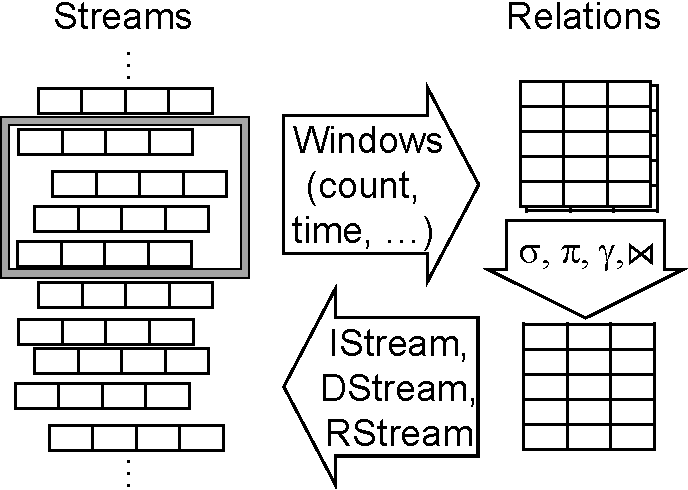
\includegraphics[scale=0.5]{cqlops.pdf}}
\vspace*{-4mm}
\caption{\label{fig:cqlops}CQL algebra operators.}
\end{figure}

In 2004, Arasu et al.\ at Stanford introduced CQL (for Continuous
Query Language)~\cite{arasu_widom_2004}. CQL has been designed as an
SQL-based declarative language for implementing continuous queries
against streams of data, such as the LinearRoad
benchmark~\cite{arasu_et_al_2004}. The design was influenced by the
TelegraphCQ system, which proposed an SQL-based language with a
focus on expressive windowing
constructs~\cite{chandrasekaran_et_al_2003}.
Figure~\ref{fig:cql} illustrates a CQL code example that
uses a time-sliding window (per minute within the last 24 hours) over
phone calls to return the maximum phone call length along with its
count and caller information.

The semantics of CQL are
based on two phases of data, \emph{streams} and \emph{relations}.
As Figure~\ref{fig:cqlops} illustrates, CQL
supports three classes of operators over these types. First,
\emph{stream-to-relation} operators produce a relation from a
stream.  The design of these operators is based on the concept of a
\emph{window} over a stream, which, at any point of time, contains a
historical snapshot of a recent portion of the stream. CQL includes
time-based and tuple-based windows, both with optional
partitioning. Second, \emph{relation-to-relation} operators, which
produce a relation from other relations. These operators are expressed
using standard SQL syntax and come from traditional relational
algebra, such as select~($\sigma$), project~($\pi$),
group-by-aggregate~($\gamma$), and join~($\bowtie$).
Third, \emph{rela\-tion-to-stream} operators, which produce a
stream from a relation. CQL supports three operators of this class:
IStream, DStream, and RStream (to capture inserts, deletes, or the entire
relation).  CQL has influenced the design of many
systems, for example, Microsoft StreamInsight~\cite{ali_et_al_2009}.

GSQL~\cite{cranor_et_al_2003} is another streaming  language with SQL-like syntax.
It has been designed in the context of the Gigascope system~\cite{cranor2003gigascope}, a stream database for network applications
including traffic analysis, intrusion detection, router configuration
analysis, and network monitoring.
In GSQL, all queries operate over streams, as inputs and outputs. 
In addition to the standard SQL operators (e.g., $\sigma$, $\pi$,
$\gamma$,~$\bowtie$), GSQL supports the \emph{merge} operator that
combines streams from multiple sources in order as specified by
ordered attributes.
GSQL supports the join of two streams as long as it can determine
a join window from the join predicates. However, GSQL does
not support the join of a stream to a non-stream relation.
